\subsection{Work sharing}

\textbf{Work-sharing constructs divide the execution of a region of code among the team members who encounter it}. A work-sharing construct must be enclosed in a parallel region for the directive to be executed in parallel. Note that the \textbf{constructs do not start new threads}. Also, there is \textbf{\underline{no} implicit barrier at the \emph{entry}} of a work-sharing construct, but \textbf{\underline{there is} an implicit barrier at the \emph{exit}} of a work-sharing construct.

\longline

\subsubsection{For}

The for directive \textbf{shares iterations of a loop across the team} (data parallelism).
\begin{figure}[!htp]
    \centering
    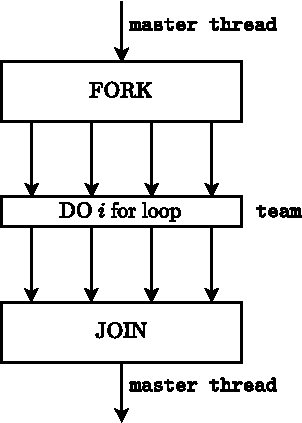
\includegraphics[width=.3\textwidth]{img/openmp-for-1.pdf}
    \caption{OpenMP for loop.}
\end{figure}

\noindent
\begin{openmpbox}[: \texttt{pragma omp for}]
\begin{lstlisting}[language=C++]
#pragma omp parallel
{
    #pragma omp for
    /* for loop */
}\end{lstlisting}
\end{openmpbox}

\noindent
The for directive parallelize execution of iterations. The number of iteration cannot be internally modified. Some common clauses are:
\begin{itemize}
    \item \texttt{\emph{schedule}} that describes \textbf{how iterations of the loop are distributed among the threads in the team}. The schedule type can be either \texttt{dynamic}, \texttt{guided}, \texttt{runtime}, or \texttt{static}.
    \begin{itemize}
        \item \texttt{\emph{static}}. Loop \textbf{iterations are divided into blocks of size \texttt{chunk}} and then statically allocated to threads. If \texttt{chunk} is \textbf{\underline{not} specified}, the \textbf{iterations are divided evenly} (if possible) \textbf{among the threads}.
        \newpage
        \begin{openmpbox}[: \texttt{static schedule}]
\begin{lstlisting}[language=C++, mathescape=true]
#pragma omp for schedule(static, $\emph{chunk-size}$)\end{lstlisting}
        \end{openmpbox}
        \begin{figure}[!htp]
            \centering
            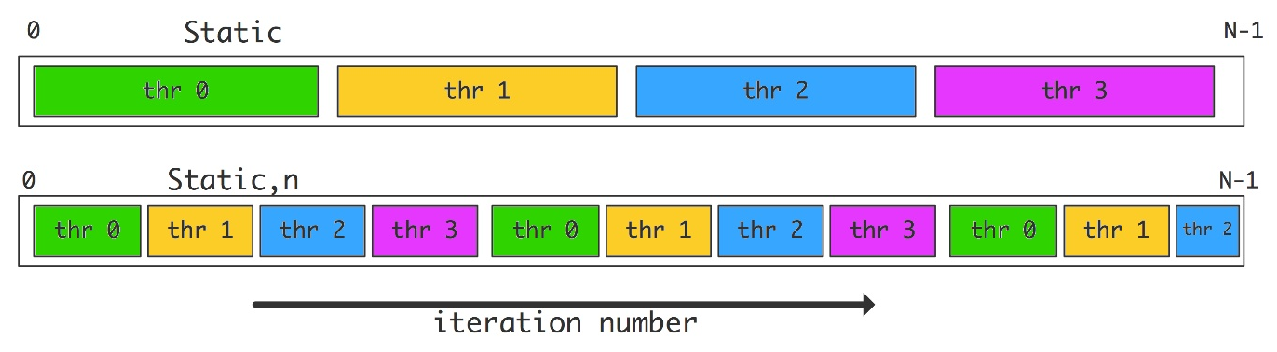
\includegraphics[width=\textwidth]{img/openmp-for-2.pdf}
            \caption{\texttt{static} schedule.}
        \end{figure}

        \item \texttt{\emph{dynamic}}. Loop \textbf{iterations are divided into blocks of size \texttt{chunk}} and \textbf{distributed among the threads \emph{at runtime}}; when a thread completes one chunk, it is \textbf{dynamically allocated another}. The default chunk size is 1. In fact, we can see in the image that the order is not always the same.
        \begin{openmpbox}[: \texttt{dynamic schedule}]
\begin{lstlisting}[language=C++, mathescape=true]
#pragma omp for schedule(dynamic, $\emph{chunk-size}$)\end{lstlisting}
        \end{openmpbox}
        \begin{figure}[!htp]
            \centering
            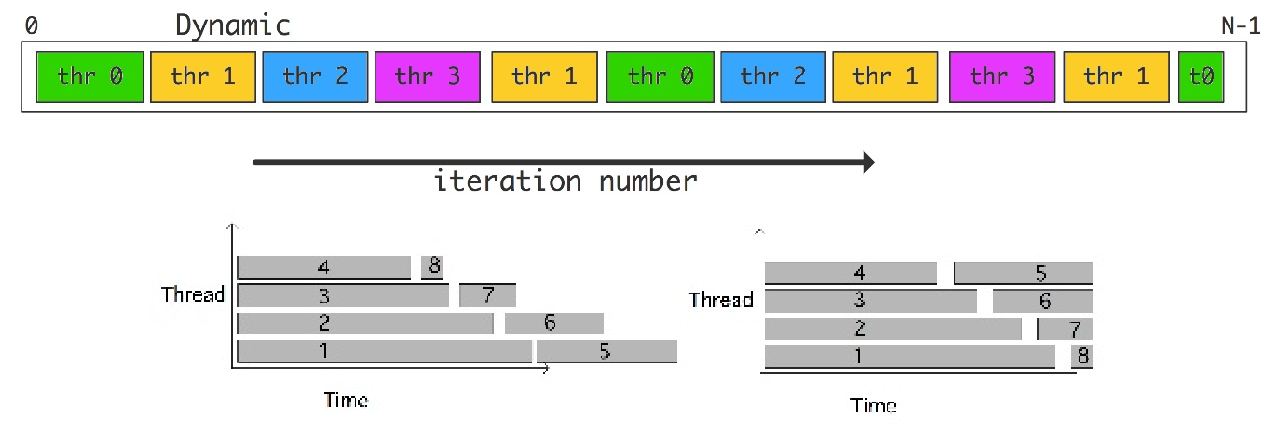
\includegraphics[width=\textwidth]{img/openmp-for-3.pdf}
            \caption{\texttt{dynamic} schedule.}
        \end{figure}
        
        \item \texttt{\emph{runtime}}. Depends on environment variable \texttt{OMP\_SCHEDULE}.

        \item \texttt{\emph{guided}}. Static, gradually decreases the chunk size (\texttt{chunk} specifies the smallest one).
        \begin{openmpbox}[: \texttt{guided schedule}]
\begin{lstlisting}[language=C++, mathescape=true]
#pragma omp for schedule(guided)\end{lstlisting}
        \end{openmpbox}
        \begin{figure}[!htp]
            \centering
            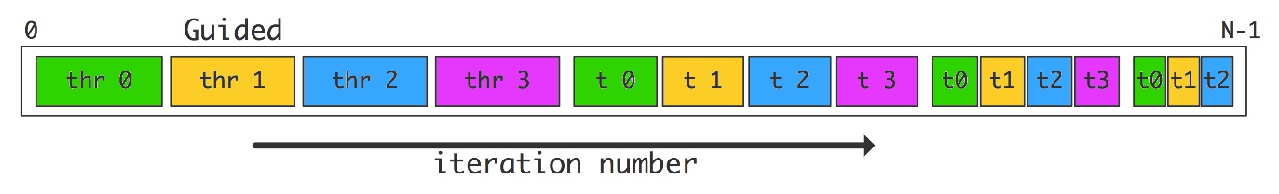
\includegraphics[width=\textwidth]{img/openmp-for-4.pdf}
            \caption{\texttt{guided} schedule.}
        \end{figure}
    \end{itemize}
    \begin{examplebox}[: \texttt{schedule} types]
\begin{lstlisting}[language=C++]
#include <stdio.h>
#include <omp.h>

#define NUM_THREADS 4
#define STATIC_CHUNK 5
#define DYNAMIC_CHUNK 5
#define NUM_LOOPS 20
#define SLEEP_EVERY_N 3

int main( )
{
    int nStatic1[NUM_LOOPS],
        nStaticN[NUM_LOOPS];
    int nDynamic1[NUM_LOOPS],
        nDynamicN[NUM_LOOPS];
    int nGuided[NUM_LOOPS];

    omp_set_num_threads(NUM_THREADS);

    #pragma omp parallel
    {
        #pragma omp for schedule(static, 1)
        for (int i = 0 ; i < NUM_LOOPS ; ++i)
        {
            if ((i % SLEEP_EVERY_N) == 0)
                Sleep(0);
            nStatic1[i] = omp_get_thread_num( );
        }

        #pragma omp for schedule(static, STATIC_CHUNK)
        for (int i = 0 ; i < NUM_LOOPS ; ++i)
        {
            if ((i % SLEEP_EVERY_N) == 0)
                Sleep(0);
            nStaticN[i] = omp_get_thread_num( );
        }

        #pragma omp for schedule(dynamic, 1)
        for (int i = 0 ; i < NUM_LOOPS ; ++i)
        {
            if ((i % SLEEP_EVERY_N) == 0)
                Sleep(0);
            nDynamic1[i] = omp_get_thread_num( );
        }

        #pragma omp for schedule(dynamic, DYNAMIC_CHUNK)
        for (int i = 0 ; i < NUM_LOOPS ; ++i)
        {
            if ((i % SLEEP_EVERY_N) == 0)
                Sleep(0);
            nDynamicN[i] = omp_get_thread_num( );
        }

        #pragma omp for schedule(guided)
        for (int i = 0 ; i < NUM_LOOPS ; ++i)
        {
            if ((i % SLEEP_EVERY_N) == 0)
                Sleep(0);
            nGuided[i] = omp_get_thread_num( );
        }
    }

    printf_s("------------------------------------------------\n");
    printf_s("| static | static | dynamic | dynamic | guided |\n");
    printf_s("|    1   |    %d   |    1    |    %d    |        |\n",
                STATIC_CHUNK, DYNAMIC_CHUNK);
    printf_s("------------------------------------------------\n");

    for (int i=0; i<NUM_LOOPS; ++i)
    {
        printf_s("|    %d   |    %d   |    %d    |    %d    |"
                    "    %d   |\n",
                    nStatic1[i], nStaticN[i],
                    nDynamic1[i], nDynamicN[i], nGuided[i]);
    }

    printf_s("------------------------------------------------\n");
}\end{lstlisting}
    The result will be:
\begin{lstlisting}
------------------------------------------------
| static | static | dynamic | dynamic | guided |
|    1   |    5   |    1    |    5    |        |
------------------------------------------------
|    0   |    0   |    0    |    2    |    1   |
|    1   |    0   |    3    |    2    |    1   |
|    2   |    0   |    3    |    2    |    1   |
|    3   |    0   |    3    |    2    |    1   |
|    0   |    0   |    2    |    2    |    1   |
|    1   |    1   |    2    |    3    |    3   |
|    2   |    1   |    2    |    3    |    3   |
|    3   |    1   |    0    |    3    |    3   |
|    0   |    1   |    0    |    3    |    3   |
|    1   |    1   |    0    |    3    |    2   |
|    2   |    2   |    1    |    0    |    2   |
|    3   |    2   |    1    |    0    |    2   |
|    0   |    2   |    1    |    0    |    3   |
|    1   |    2   |    2    |    0    |    3   |
|    2   |    2   |    2    |    0    |    0   |
|    3   |    3   |    2    |    1    |    0   |
|    0   |    3   |    3    |    1    |    1   |
|    1   |    3   |    3    |    1    |    1   |
|    2   |    3   |    3    |    1    |    1   |
|    3   |    3   |    0    |    1    |    3   |
------------------------------------------------\end{lstlisting}
    \end{examplebox}

    \item \texttt{\emph{nowait}} to \textbf{avoid synchronization at the end of the parallel loop}. It overrides the barrier implicit in a directive.
    \begin{lstlisting}[language=C++]
#pragma omp for nowait\end{lstlisting}
    \begin{examplebox}[: \texttt{nowait} clause]
\begin{lstlisting}[language=C++]
#include <stdio.h>

#define SIZE 5

void test(int *a, int *b, int *c, int size)
{
    int i;
    #pragma omp parallel
    {
        #pragma omp for nowait
        for (i = 0; i < size; i++)
            b[i] = a[i] * a[i];

        #pragma omp for nowait
        for (i = 0; i < size; i++)
            c[i] = a[i]/2;
    }
}

int main( )
{
    int a[SIZE], b[SIZE], c[SIZE];
    int i;

    for (i=0; i<SIZE; i++)
        a[i] = i;

    test(a,b,c, SIZE);

    for (i=0; i<SIZE; i++)
        printf_s("%d, %d, %d\n", a[i], b[i], c[i]);
}\end{lstlisting}
    The output will be:
\begin{lstlisting}
0, 0, 0
1, 1, 0
2, 4, 1
3, 9, 1
4, 16, 2\end{lstlisting}
    \end{examplebox}
\end{itemize}

\newpage

\paragraph{Reduction}\label{paragraph: Reduction}

\noindent
In parallel programming, sometimes there are some exceptional cases when we use the \texttt{for} statement where the variables inside the code block are not so easy to manage (memory viewpoint). For example, consider the following case:
\begin{center}
\begin{lstlisting}[language=C++]
#include "stdio.h"
#include "omp.h"
#define MAX 10


int main(int argc, char const *argv[])
{
    double ave = 0.0;
    double A[MAX] = {1, 2, 3, 4, 5, 6, 7, 8, 9, 10};
    int i;
    #pragma omp parallel for
    for(i = 0; i < MAX; i++) {
        ave += A[i];
    }
    ave = ave / MAX;
    printf("Value %f\n", ave);
    return 0;
}
\end{lstlisting}
\textcolor{Red2}{\faIcon{exclamation-triangle} \textbf{Too many threads modifying the same variable}}
\end{center}
In this case, we are combining values into a single accumulation variable (called \texttt{ave}). There is a true dependence between loop iterations that can't be trivially removed. A \textbf{continuous execution produces different results!}
\begin{lstlisting}[language=bash, mathescape=false]
$ ./example.out
Value 1.300000
$ ./example.out
Value 2.400000
$ ./example.out 
Value 2.500000
$ ./example.out 
Value 2.100000
$ ./example.out 
Value 1.900000    
\end{lstlisting}
This is a very common situation and a solution, which can also be \textbf{used as a synchronization technique}, is called a \textbf{reduction}.

\highspace
A reduction variable in a loop \textbf{aggregates} (i.e., accumulates) a \textbf{value that depends on each iteration of the loop} and \textbf{doesn't depend on the iteration order}.

\begin{openmpbox}[: \texttt{reduction}]
    \begin{lstlisting}[language=C++, mathescape=true]
#pragma omp parallel for reduction($\emph{operator}$: $\emph{list}$)\end{lstlisting}
\end{openmpbox}

\noindent
A reduction clause:
\begin{itemize}
    \item It \textbf{makes a local copy} of each \texttt{\emph{list}} variable and initialized depending on the \texttt{\emph{operator}};
    \item It \textbf{updates occur on the local copy};
    \item \textbf{Local copies are reduced into a single value and combined with the original global value}.
\end{itemize}
Therefore, the variables in \texttt{\emph{list}} must be shared in the enclosing parallel region.

\highspace
Many different associative operands (\texttt{\emph{operator}} value) can be used with reduction:
\begin{itemize}
    \item \texttt{+} with initial value 0
    \item \texttt{*} with initial value 1
    \item \texttt{-} with initial value 0
    \item \texttt{min} with initial value as largest positive number
    \item \texttt{max} with initial value as most negative number
    \item \texttt{\&} with initial value $\sim0$
    \item \texttt{|} with initial value 0
    \item \texttt{\textasciicircum} with initial value 0
    \item \texttt{\&\&} with initial value 1
    \item \texttt{||} with initial value 0
\end{itemize}
Using the \texttt{reduction} clause, the code written at the beginning of the paragraph can be fixed as follows:
\begin{center}
\begin{lstlisting}[language=C++]
#include "stdio.h"
#include "omp.h"
#define MAX 10


int main(int argc, char const *argv[])
{
    double ave = 0.0;
    double A[MAX] = {1, 2, 3, 4, 5, 6, 7, 8, 9, 10};
    int i;
    // use reduction
    #pragma omp parallel for reduction(+: ave)
    for(i = 0; i < MAX; i++) {
        ave += A[i];
    }
    ave = ave / MAX;
    // now it prints the correct result 5.5
    printf("Value %f\n", ave);
    return 0;
}
\end{lstlisting}
\textcolor{Green3}{\faIcon{check} \textbf{Avoid race condition}}
\end{center}

\newpage

\subsubsection{Sections}

\textbf{Section} identifies code \textbf{sections to be divided among all threads}.

\highspace
Sections allow to specify that the enclosed section(s) of code are to be executed in parallel. \textbf{Each section is executed once by a thread in the team}.

\marginpar{
    \href{https://www.openmp.org/spec-html/5.0/openmpsu37.html\#x59-1010002.8.1} {Doc. \faIcon{book}}
}
\begin{openmpbox}[: sections]
\begin{lstlisting}[language=C++]
#pragma omp [parallel] sections [clauses]
{
    #pragma omp section
    {
        code_block
    }
}\end{lstlisting}
\end{openmpbox}

\noindent
The sections directive identifies a noniterative work-sharing construct that specifies a set of constructs that are to be divided among threads in a team. Each section is executed once by a thread in the team.

\highspace
Each section is preceded by a \texttt{section} directive, although the \texttt{section} directive is optional for the first section. The \texttt{section} directives must appear within the lexical extent of the \texttt{sections} directive. There's an \textbf{implicit barrier} at the end of a \texttt{sections} construct, unless a \texttt{nowait} is specified.

\highspace
Restrictions to the sections directive are as follows:
\begin{itemize}
    \item A \texttt{section} directive must not appear outside the lexical extent of the \texttt{sections} directive.
    \item Only a single \texttt{nowait} clause can appear on a \texttt{sections} directive.
\end{itemize}

\begin{figure}[!htp]
    \centering
    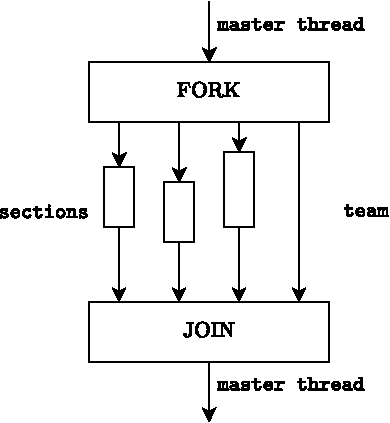
\includegraphics[width=.45\textwidth]{img/openmp-sections-1.pdf}
    \caption{Breaks work into separate, discrete sections, each executed by a thread (functional parallelism).}
\end{figure}

\newpage

\subsubsection{Single/Master}

A \textbf{section} (not the directive) \textbf{of code should be executed on a single thread, not necessarily the main (master) thread}. The \texttt{single} directive identifies a construct that specifies that the associated structured block is executed by only one thread in the team (not necessarily the master thread).

\begin{openmpbox}[: \texttt{single} and \texttt{master}]
\begin{lstlisting}[language=C++]
#pragma omp parallel
{
    #pragma omp single
    {
        /* code section */
    }
    # pragma omp master
    {
        /* code section */
    }
}\end{lstlisting}
\end{openmpbox}

\begin{itemize}
    \item \texttt{single} specifies that a section of a code is \textbf{executed only by a single thread}.\marginpar{
        \href{https://www.openmp.org/spec-html/5.0/openmpsu38.html\#x60-1090002.8.2} {Doc. \faIcon{book}}
    }

    
    \item \texttt{master} specifies that a section of a code is \textbf{executed only by the master}.\marginpar{
        \href{https://www.openmp.org/spec-html/5.0/openmpse24.html\#x118-4380002.16} {Doc. \faIcon{book}}
    }
\end{itemize}

\noindent
There's an \textbf{implicit barrier} after the \texttt{single} construct unless a \texttt{nowait} clause is specified.

\newpage

\subsubsection{Tasks}

The following section has been enhanced with slides from Senior Principal Engineer Mattson Tim. He's a senior principal engineer at Intel, where he's been since 1993. His profile can be seen \href{https://www.intel.com/content/www/us/en/research/featured-researchers/tim-mattson.html}{here} and the slides are available online \href{https://www.openmp.org/wp-content/uploads/Intro_To_OpenMP_Mattson.pdf}{here}. He has also made an interesting \href{https://youtube.com/playlist?list=PLLX-Q6B8xqZ8n8bwjGdzBJ25X2utwnoEG&si=OBjyY4AI4zWfA-vB}{YouTube series} on the introduction to OpenMP.

\highspace
Tasks are \textbf{independent units of work}. They consist of: \emph{code to execute}, \emph{data environment}, and \emph{internal control variables} (ICV). \textbf{Threads perform the work of each task}. The runtime \textbf{system decides when to execute tasks}; each task can be deferred or executed immediately.

\highspace
Some useful terminology:
\begin{itemize}
    \item \textbf{\emph{Task construct}}. It identifies the \textbf{task directive plus the structured block}.
    
    \item \textbf{\emph{Task}}. It is the \textbf{package of code and instructions} for \textbf{allocating data} created when a \textbf{thread encounters a task construct}.
    
    \item \textbf{\emph{Task region}}. It is the dynamic sequence of \textbf{instructions generated by the execution of a task by a thread}.
\end{itemize}
Tasks are guaranteed to complete at thread barriers (using the \texttt{barrier} directive) or at task barriers (using the \texttt{taskwait} directive):
\begin{lstlisting}[language=C++, mathescape=true]
#pragma omp parallel // omp directive to parallel the code
{
    #pragma omp task // multiple $\textcolor{codegreen}{\emph{foo}}$ tasks created here, 
                     // one for each thread
    foo();
    #pragma omp barrier // all $\textcolor{codegreen}{\emph{foo}}$ tasks guaranteed 
                        // to be completed here
    #pragma omp single  // only one thread can access to 
                        // this piece of code
    {
        #pragma omp task // one $\textcolor{codegreen}{\emph{bar}}$ task created here
        bar();
    }
    // $\textcolor{codegreen}{\emph{foo}}$ task guaranteed to be completed here
}
\end{lstlisting}
\begin{examplebox}[: Fibonacci with tasks]
    Let us see a Fibonacci example of data scoping using the tasks. In the following code, we create the Fibonacci function and we create two tasks, but each task has a private variable and these variables are also used in the return statement:
    \begin{lstlisting}[language=C++]
int fib(int n) {
    int x, y;
    if(n < 2)
        return n;
    #pragma omp task
    x = fib(n-1);
    #pragma omp task
    y = fib(n-2);
    #pragma omp taskwait
    return x + y;
}\end{lstlisting}
    A good solution is to \dquotes{share} the \texttt{x} and \texttt{y} variables because we need both values to calculate the sum.
    \begin{lstlisting}[language=C++]
int fib(int n) {
    int x, y;
    if(n < 2)
        return n;
    #pragma omp task shared(x)
    x = fib(n-1);
    #pragma omp task shared(y)
    y = fib(n-2);
    #pragma omp taskwait
    return x + y;
}\end{lstlisting}
\end{examplebox}

\begin{flushleft}
    \textcolor{Green3}{\faIcon{check} \textbf{Main advantage}}
\end{flushleft}
Note the following code:
\begin{lstlisting}[language=C++]
// create a team of threads
#pragma omp parallel
{
    // one thread executes the single construct
    // and other threads wait at the implied 
    // barrier at the end of the single construct
    #pragma omp single
    { // block 1
        node *p = head;
        while(p) { // block 2
            // the single thread creates a task
            // with its own value for the pointer p
            #pragma omp task firstprivate(p)
                process(p);
            p = p -> next; // block 3
        }
        // execution moves beyond the barrier 
        // once all the tasks are complete
    }
}
\end{lstlisting}
The tasks have the \textbf{potential to parallelize irregular patterns and recursive function calls}. See Figure \ref{figure: openmp tasks 1} (page \pageref{figure: openmp tasks 1}) to understand how the runtime system can optimize execution using the tasks.
\begin{figure}[!htp]
    \centering
    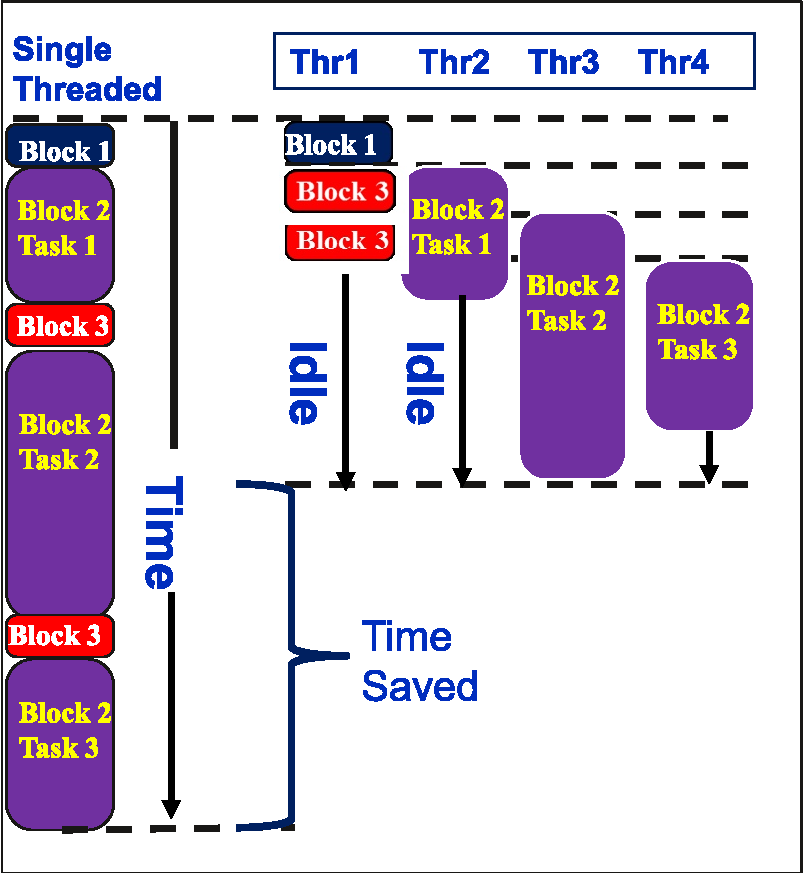
\includegraphics[width=.6\textwidth]{img/openmp-tasks-1.pdf}
    \caption{The main advantage of the tasks is to parallelize irregular patterns and recursive function calls.}
    \label{figure: openmp tasks 1}
\end{figure}